% Whole-project synthesis. Source snapshot 6ee4199; application equals dev0e43bcb.
\section{Thiết kế dữ liệu và hợp đồng API}
\label{sec:data-api}
\subsection{Từ domain model đến mô hình quan hệ thực tế}
Domain Class Diagram ở chương trước diễn tả khái niệm nghiệp vụ; mô hình lưu
trữ thực tế được đối chiếu từ \path{apps/api/prisma/schema.prisma} và SQL
trong \path{apps/api/prisma/migrations}. Snapshot ứng dụng có 13 Prisma models,
12 enum và 10 migrations. Các ghi chú đề xuất cũ trong header schema hoặc DBML
không thay thế trạng thái của các migration đã có. Đó là bằng chứng source
\textbf{Implemented}, chưa xác nhận migration state của database production.

\begin{longtable}{>{\raggedright\arraybackslash}p{0.27\linewidth}>{\raggedright\arraybackslash}p{0.63\linewidth}}
\caption[Mô hình quan hệ từ schema thực tế]{Mô hình quan hệ từ schema thực tế}\label{tab:relational-model}\\
\toprule Nhóm bảng & Quan hệ và ý nghĩa lưu trữ \\ \midrule
\endfirsthead
\toprule Nhóm bảng & Quan hệ và ý nghĩa (tiếp) \\ \midrule \endhead
Category, Product & Một category có nhiều product; mỗi product thuộc một category.
Product lưu giá gốc VND, stock, size policy và dữ liệu hiển thị. \\
Topping, ProductTopping & Product--Topping là N:M qua khóa ghép; catalog kiểm soát
topping hợp lệ theo từng sản phẩm, không mặc định mọi topping dùng cho mọi món. \\
User, Order & Một user có nhiều order; order giữ tổng trước/sau giảm giá,
trạng thái và thời điểm hết hạn/thanh toán. User giữ số điểm hiện hành. \\
OrderItem, OrderItemTopping & Order có nhiều dòng. Tên/giá sản phẩm, size và giá
topping được snapshot để lịch sử đơn không phụ thuộc giá catalog thay đổi. \\
Coupon, CouponRedemption & Redemption liên kết user/coupon/order, với trạng thái
HELD, CONSUMED, RELEASED; unique orderId giới hạn tối đa một redemption/order. \\
Payment, PaymentGatewayEvent & Order có nhiều payment attempt; payment thuộc user.
Event ghi nguồn IPN/QUERYDR, outcome và disposition để xử lý trùng/xung đột. \\
SeedExecution & Marker hoàn tất một seed version; migration10 bổ sung bảng này,
không phải dữ liệu nghiệp vụ thanh toán. \\
\bottomrule
\end{longtable}

FK nghiệp vụ chủ yếu dùng Restrict; liên kết catalog ProductTopping dùng Cascade.
Tiền được lưu BigInt VND, không dùng floating point để quyết định tổng đơn.
SQL migrations còn chứa CHECK và partial unique indexes không thể hiện hết
trong một domain diagram: stock/giá/điểm không âm, quantity 1--10,
lineTotal = unitPrice $\times$ quantity, discount không vượt subtotal và
total = subtotal $-$ discount. Unique email, coupon code và các khóa liên kết
chặn trùng ở DB, bổ sung cho validation ở API.

Hai partial unique indexes quan trọng giới hạn một active order/user
(PENDING hoặc PAYMENT\_FAILED) và một payment SUCCESS/order. Payment có unique
(userId, idempotencyKey); gateway event có unique (paymentId, source,
eventIdentity). Đây là lớp bảo vệ cuối khi request hoặc callback chạy đồng
thời. Transaction và locking trong service vẫn cần thiết; có index không
chứng minh mọi concurrency scenario đã được kiểm thử ở A2.

Thiết kế có khái niệm Promotion/LoyaltyTransaction nhưng schema hiện dùng
Coupon/CouponRedemption và User.loyaltyPoints/Order.pointsEarned, chưa có
model LoyaltyTransaction riêng. Báo cáo giữ sự khác nhau này; không vẽ thêm
bảng đã triển khai hoặc suy ra đã có ledger đầy đủ (xem FR-29/FR-45 và matrix).

\subsection{API boundary, phiên bản và phân quyền}
API REST/JSON nối UI với nghiệp vụ server. Contract v1 là baseline catalog
lịch sử; v3/v4 và các addendum trong archive cung cấp quy tắc mở rộng.
V4 có caveat tổng thể NOT APPROVED/external dependencies open dù ghi riêng
API design baseline đã xác nhận trong Scope. Vì vậy dùng quy tắc normative
đã ghi cùng SRS/decision, không gọi toàn bộ contract hoặc implementation là
Approved. Danh mục dưới là inventory controller hiện có, không phải API mới.

\begin{longtable}{>{\raggedright\arraybackslash}p{0.37\linewidth}>{\raggedright\arraybackslash}p{0.53\linewidth}}
\caption[Các API chính và trust boundary]{Các API chính và trust boundary trong source}\label{tab:api-inventory}\\
\toprule Method / route & Trách nhiệm và bảo vệ \\ \midrule
\endfirsthead
\toprule Method / route & Trách nhiệm và bảo vệ (tiếp) \\ \midrule \endhead
GET /products; GET /products/:id & Public catalog/list/detail; không lấy UI làm
nguồn giá có thẩm quyền khi tạo order. \\
POST /auth/register; POST /auth/login & DTO validation, chuẩn hóa email và
Argon2id; login phát JWT, không trả password hash. \\
GET /auth/me & JwtAuthGuard, lấy identity từ token được xác minh. \\
POST /orders; GET /orders/me & JWT; service kiểm ownership, tính lại giá và
điều phối tài nguyên; history chỉ thuộc Customer hiện tại. \\
POST /coupons/preview & JWT; preview không giữ quota, validation tạo order vẫn
là bước có thẩm quyền. Scope acceptance FR-43 cần quyết định riêng. \\
POST /payments; POST /payments/vnpay/initiate & JWT, ownership, idempotency;
Mock còn chịu environment/access guard, không bật cho production. \\
GET /payments/vnpay/ipn & Callback gateway không dùng Customer JWT; xác minh
chữ ký và dữ liệu giao dịch trước shared finalization. \\
POST /internal/orders/:id/advance & InternalKeyGuard và DTO from; chuyển một
bước PAID--PREPARING--READY--COMPLETED. Không phải UI Admin/Barista đã bàn giao. \\
GET / & Public liveness, trả Hello World!; không query DB. \\
\bottomrule
\end{longtable}

Controller nhận request, DTO/Guard chặn dữ liệu hoặc danh tính không hợp lệ,
service quyết định nghiệp vụ và Prisma thực hiện truy cập/transaction.
Ownership lấy từ JWT, không tin userId do client tự chọn. Business conflict,
not-found và validation phải theo contract; báo cáo không tự bổ sung status
code/error code. Gap API-03 payment-status được phân tích ở phần kiểm thử;
không liệt kê route đó như API đã implemented.

\section{Hiện thực hệ thống BrewLite}
\label{sec:implementation}
\subsection{Frontend và hành trình người dùng}
App Router tại \path{apps/web/app} cung cấp menu, product detail, login/register,
payment, order confirmation và history. React Context quản lý auth/cart;
services tách việc gọi API khỏi component. Các request thông thường đi qua
Route Handler \path{apps/web/app/api/backend/[[...path]]/route.ts} để server
Next.js forward tới NestJS. Target ưu tiên BACKEND\_INTERNAL\_URL rồi
NEXT\_PUBLIC\_API\_URL; tên biến không biến kết nối Vercel--Render thành private.
Proxy đã được PR16 harden response headers và thông báo lỗi upstream chung.

Menu thể hiện loading/empty/error và lọc category; modal cho chọn size/topping,
quantity và giỏ. Checkout dùng catalog preview để hỗ trợ người dùng nhưng
server tính giá cuối. Auth state/token được lưu localStorage theo source
hiện hành; Bearer JWT được gửi tới API. Cách này đơn giản cho client nhưng
token chịu rủi ro khi có XSS, không phải HttpOnly-cookie authentication.
Responsive breakpoints có trong code; chưa có manifest/service worker hoặc
bằng chứng installability để ghi PWA đã Verified.

\begin{figure}[htbp]
\centering
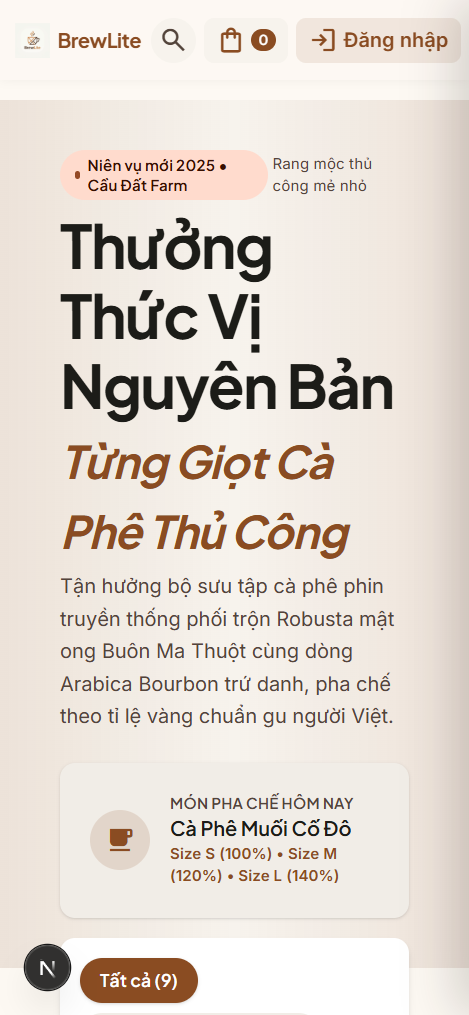
\includegraphics[height=0.48\textheight]{docs/A2_TestReport/evidence/menu_375x812.png}
\hspace{10mm}
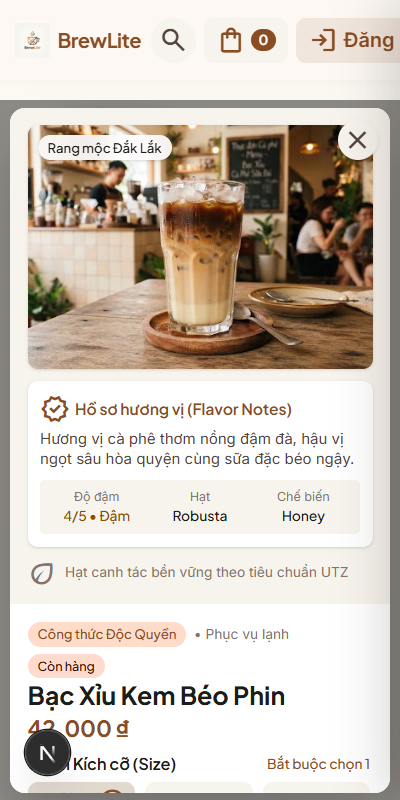
\includegraphics[height=0.48\textheight]{docs/A2_TestReport/evidence/modal_320x640_top.png}
\caption[Giao diện local lịch sử SCRUM-112]{Ảnh local lịch sử SCRUM-112: đầu trang menu 375x812 và phần trên modal
320x640. Nguồn report kiểm source34cbbc0; không phải ảnh production hiện tại.
Modal là viewport có cuộn, không biểu diễn toàn bộ form trong một ảnh.}
\label{fig:historical-ui}
\end{figure}

Các ảnh trên minh họa tạo phẩm UI thực đã tồn tại; không thay một demo toàn
luồng từ menu tới confirmation. Ảnh không có credential và được mở kiểm tra
trước khi tích hợp. Những điều kiện validation/trạng thái cụ thể tiếp tục
truy về SRS/use case và test inventory, không suy từ một màn hình đẹp.

\subsection{Backend, transaction và các luồng chính}
AppModule hiện import Products, Auth, Orders, Payments và Coupons. Inventory,
promotion/loyalty và reconciliation là các trách nhiệm domain được điều phối
trong modular monolith, không phải mỗi khái niệm đều có service deploy riêng.
Mô tả A1 cũ nói Orders/Payments chưa nằm trong AppModule đã lỗi thời khi áp
dụng cho A2; báo cáo này cập nhật từ source6ee4199/app baseline0e43bcb.

Luồng tạo đơn bắt đầu bằng JWT/validation, đọc lựa chọn catalog, tính giá
server-side, khóa/kiểm tài nguyên, giữ stock và coupon trong transaction rồi
tạo Order/OrderItem snapshots. Thiếu stock hoặc lỗi phải rollback cả đơn và
side effects. Backend lưu expiry; expiration giải phóng tài nguyên theo state
machine thay vì mặc định cho Customer hủy chủ động.

Luồng thanh toán kiểm owner, số tiền và idempotency. ZERO\_AMOUNT, Mock và
VNPay hội tụ tại shared finalization để tránh lặp cập nhật Order/stock/coupon/
loyalty. Return URL chỉ đưa người dùng về UI; IPN hoặc kết quả QueryDR được
xác minh mới có thể dẫn tới kết quả tài chính có thẩm quyền. Unknown/timeout
không tự đồng nghĩa FAILED. Order PAID không bị trả về PENDING bởi callback
trùng; callback xung đột hoặc quá hạn cần cơ chế financial exception/review.

Expiration và reconciliation scheduler là timer cùng vòng đời NestJS process.
Sleep/restart và nhiều instance vì vậy ảnh hưởng vận hành, chưa được chứng
minh chỉ bằng source. Các quy tắc grace/late payment/ZERO\_AMOUNT chi tiết giữ
theo contract và sequence đã trình bày, không thêm transition trong báo cáo.

\subsection{Bảo mật, validation và những sai khác cần giữ rõ}
JWT HS256/expiry và UUID sub được kiểm phía server; service kiểm ownership.
Auth dùng Argon2id, DTO validation theo endpoint; internal order advancement
cần internal key. Không đồng nhất cơ chế internal key với quyền Customer.
Secrets JWT/VNPay/DB ở environment backend; ảnh và log sử dụng evidence đã lọc.
SCRUM-117 không đọc giá trị environment thật để suy ra cấu hình production.

Một sai khác đã được MVP report nêu và còn trong source: FE
\path{apps/web/services/api.service.ts} tính size price bằng floor, trong khi
SRS/API và \path{apps/api/src/orders/cart-pricing.ts} dùng round-half-up.
Ví dụ giá35004, hệ số120\% cho preview42004 nhưng backend42005 VND.
Seed giá chẵn có thể che sai khác này. Server giữ giá cuối nhưng UI preview
có thể lệch1 VND ở một số giá; cần task sửa và regression test được duyệt.
Không sửa code hoặc tự waive FR-11 trong task báo cáo.

Nguồn chương: schema/migrations và các controller/service trong
\path{apps/api/src}; routes/components/context/services trong \path{apps/web};
\path{docs/architecture/architecture.md}; API v4 và MVP report. Các vị trí
code/test theo từng FR/NFR nằm trong \path{docs/traceability-matrix.md}.
